% !TEX options=--shell-escape
%!TEX program = xelatex
\documentclass{article}
\usepackage{minted}
\setminted{fontsize=\footnotesize}


\usepackage{graphicx}
\graphicspath{{image/}{figure/}{fig/}{img/}}
\usepackage[a4paper,margin=2.5cm]{geometry}
\usepackage[dvipsnames]{xcolor}
\usepackage{hyperref}
\hypersetup{
  colorlinks,
  citecolor=Violet,
  linkcolor=Red,
  urlcolor=NavyBlue}

\usepackage{dtk-logos}% or use package holog
  
\usepackage{xeCJK}
\usepackage{fontspec,xunicode,xltxtra}
\setmainfont{Minion Pro}
\setsansfont{Myriad Pro}
\setmonofont{Ubuntu Mono}
\setCJKmainfont[ItalicFont={方正楷体简体}, BoldFont={方正黑体简体}]{方正书宋简体}
\setCJKsansfont[BoldFont={方正黑体简体}]{方正楷体简体}
\setCJKmonofont{方正楷体简体}

\usepackage{indentfirst}
\setlength{\parindent}{2em}

\usemintedstyle{elegant}
\linespread{1.3}
\usepackage{etoolbox,xpatch}

\makeatletter
\AtBeginEnvironment{minted}{\dontdofcolorbox}
\def\dontdofcolorbox{\renewcommand\fcolorbox[4][]{##4}}
\xpatchcmd{\inputminted}{\minted@fvset}{\minted@fvset\dontdofcolorbox}{}{}
\makeatother

% caption settings 
\usepackage[font=small,labelfont={bf}]{caption} 
\captionsetup[table]{skip=3pt}
\captionsetup[figure]{skip=3pt}

% list/itemize/enumerate setting
\usepackage[shortlabels]{enumitem}
\setlist{nolistsep}

\renewcommand{\figurename}{\bfseries 图}
\renewcommand{\tablename}{\bfseries 表}

\title{\bfseries \LaTeX{} 编译环境配置:Sublime Text 配置简介}
\author{\href{https://ddswhu.me/}{Dongsheng Deng}}
\date{February 6, 2019}


\begin{document}
\maketitle

本文介绍如何使用 Sublime Text 搭建 \LaTeX{} 编写环境。Github 地址:\href{https://github.com/EthanDeng/sublime-text-latex}{sublime-text-latex},欢迎提交 issues 和 pull requests。引用请注明来源!

\section{简介}
Sublime Text 是一个轻量级的、跨平台的编辑器,搭配 LaTeXTools 和 \TeX{} Live 或者 \MiKTeX 使用可以编译 \TeX{} 文件。以前你可能会觉得 LaTeX 命令很难记得住,写起来很麻烦,但是借助 Sublime Text 里面的 LaTeXTools 插件你会觉得写 \TeX{} 文档也可以是一种享受。从我自身的经验来看,自从配置好 Sublime Text 之后,我再没回去用 \TeX{}Works 或者 WinEdt。

在 2014 年,我在自己博客上发布了如何使用 Sublime Text 搭建 \LaTeX{} 编写环境,这么多年了,我的主页 发生了更迭,那篇帖子早已不见了,不过网上倒是能找到一些转载的内容。当时我将那篇帖子投稿到 \LaTeX{} Studio,有兴趣的可以看下,传送门:\href{http://www.latexstudio.net/archives/1169.html}{Sublime Text 搭建 LaTeX 编写环境}。时间过了这么多年,LaTeXTools 插件也发生了一些改变,原来的帖子感觉有点不合时代了,所以决定更新下。

\begin{figure}[htbp]
  \centering
  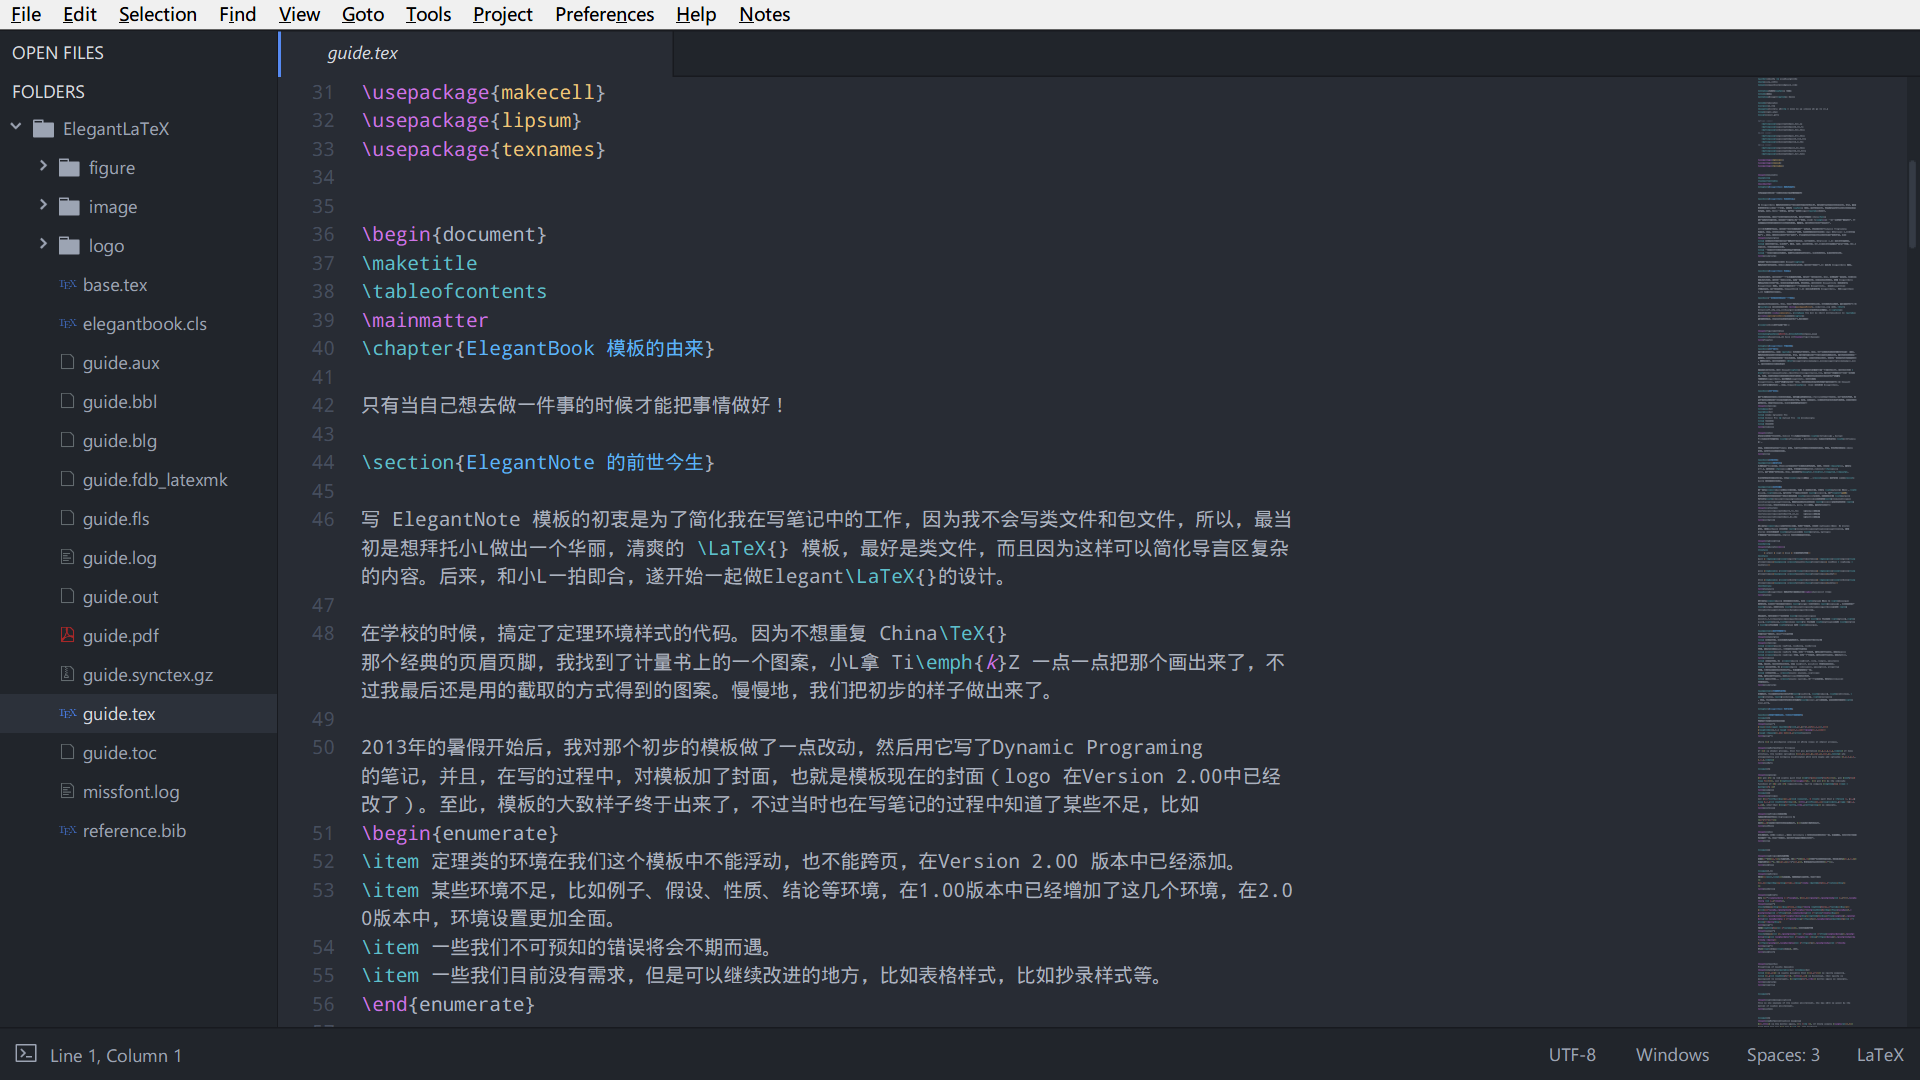
\includegraphics[width=0.9\textwidth]{sublime.png}
  \caption{Sublime Text 的界面图}
  \label{fig:sublime}
\end{figure}



\section{准备工作}
首先,为了搭建 \LaTeX{} 工作环境,你需要安装:

\begin{itemize}
  \item \TeX{} Live 或者 MiKTeX (本文以 \TeX{} Live 2018 为例)
  \item Sublime Text 3
  \item Package Control (Sublime Text 插件)
  \item LaTeXTools (Sublime Text 插件)
  \item SumatraPDF 阅读器(可选,用于预览 PDF)
\end{itemize}

\subsection{添加环境变量}

在上述软件/插件安装之后,你需要把 \TeX{} Live 的 bin 目录(\mintinline[breaklines]{shell}{D:/Program Files/texlive/2018/bin/win32}) 以及 SumatraPDF 的路径(\mintinline[breaklines]{shell}{C:/Program Files (x86)/SumatraPDF})添加到系统环境变量(\mintinline{shell}{Path})中。


\subsection{安装插件}
\subsubsection{安装 Package Control}
打开 Sublime Text 的包管理工具 \href{https://packagecontrol.io/installation}{Package Control} 的安装介绍界面,选择 Sublime Text 3 版本的安装命令(如下)并复制

\begin{minted}[frame=single,breaklines]{python}
import urllib.request,os,hashlib; h = '6f4c264a24d933ce70df5dedcf1dcaee' + 'ebe013ee18cced0ef93d5f746d80ef60'; pf = 'Package Control.sublime-package'; ipp = sublime.installed_packages_path(); urllib.request.install_opener( urllib.request.build_opener( urllib.request.ProxyHandler()) ); by = urllib.request.urlopen( 'http://packagecontrol.io/' + pf.replace(' ', '%20')).read(); dh = hashlib.sha256(by).hexdigest(); print('Error validating download (got %s instead of %s), please try manual install' % (dh, h)) if dh != h else open(os.path.join( ipp, pf), 'wb' ).write(by)
\end{minted}

然后,打开 Sublime Text,按住快捷 \mintinline{shell}{Ctrl+~}(或者 \mintinline{shell}{View -> Show Console})打开控制台,然后将上述代码粘贴到 Console 里面,完成 Package Control 的安装。

\subsubsection{安装 LaTeXTools}
在 Sublime Text 内,按住 \mintinline{shell}{Ctrl+Shift+P} 打开命令选项板(Command Palette),选择 \mintinline{shell}{Package Control: Install Package},然后找到 LaTeXTools,选择安装即可。

\subsection{添加环境变量}

Win10 中将路径添加到环境变量中的步骤如下:右键 \mintinline{shell}{我的电脑},然后选择 \mintinline{shell}{属性},在左侧选择 \mintinline{shell}{高级系统设置},然后选择下方的 \mintinline{shell}{环境变量},选择变量 \mintinline{shell}{Path} 编辑,将需要添加的路径添加进去即可。

\section{配置过程}
\subsection{配置 LaTeXTools}

改版之后的 LaTeXTools 配置起来非常方便,只需要修改用户设置文件,依次选择 \mintinline[breaklines]{shell}{Preferences -> Package Settings -> LaTeXTools -> Settings – User},打开 \mintinline{shell}{LaTeXTools.sublime-settings} 这个文件,根据自己的操作系统修改 \TeX{} 的路径(在 200 行左右),选择对应的发行版本,然后修改用于预览的 PDF 阅读器的路径(推荐 SumatraPDF,如果已经添加到系统路径,则 sumatra 不需要设置),以及指定 Sublime Text 的路径,修改之后的 \mintinline{shell}{LaTeXTools.sublime-settings} 文件如下所示

\begin{minted}[frame=single]{json}
"windows": {
  "texpath" : "D:\\Program Files\\texlive\\2017\\bin\\win32",
  "distro" : "texlive",
  "sumatra": "",
  "sublime_executable": "",
  "keep_focus_delay": 1200
},
\end{minted}

\subsection{反向搜索设置}

由于 SumatraPDF 反向搜索的选项配置是隐藏的,因此,我们这里先编译一个 \LaTeX{} 的例子,将下面的代码复制到 Sublime Text 里面

\begin{minted}[frame=single]{tex}
%!TEX program = pdflatex

\documentclass{article}

\title{test}
\author{ddswhu}
\date{\today}
 
\begin{document}
\maketitle
 
This is the context of the article.
 
\end{document}
\end{minted}

保存为 \mintinline{shell}{test.tex},再按组合键 \mintinline{shell}{Ctrl+B} 编译,SumatraPDF 就会自动弹出,显示 \mintinline{shell}{test.pdf} 的内容,然后在SumatraPDF 上方的菜单栏选择 设置,将下面的代码添加到 SumatraPDF 选项的最下面方的反向搜索设置框内即可。

\begin{minted}[frame=single]{shell}
"C:\Program Files\Sublime Text 3\sublime_text.exe" "%f:%l"
\end{minted}

确定然后关闭。这样,我们就设置好了 SumatraPDF 的反向搜索。至此,我们已经搭建好了 Sublime Text 用于编辑 \LaTeX{} 的环境。更多关于 LaTeXTools 的使用请参考官方文档或者下面的参考资料。

\section*{参考资料}
\begin{itemize}
  \item \href{https://packagecontrol.io/installation}{Package Control Installation}.
  \item \href{https://latextools.readthedocs.io/en/latest/install/}{LaTeXTools Installation}
  \item \href{https://liam.page/2013/11/11/Sublime-elegant/}{极致优雅——Sublime Text 简介/入门/技巧}
  \item \href{https://ddswhu.me/posts/2018-06/sublime-text-for-latex/}{Configure Sublime Text 3 as LaTeX IDE}
  \item \href{http://www.latexstudio.net/archives/51449.html}{LaTeX 技巧 935: Sublime Text 下的 LaTeX 及高级应用}
\end{itemize}


\end{document}
